% Digital Minds Research Sprint 2026 - submission draft
% Mirrors the official docx template structure. Upload to Overleaf as-is.
% Guidance from the template kept as % comments. Numbers marked [OK] are final
% (from results/grid_summary.json, commit-pinned); [PENDING] awaits phase 2.

\documentclass[11pt]{article}
\usepackage[a4paper, margin=2.4cm]{geometry}
\usepackage{graphicx}
\usepackage{booktabs}
\usepackage{amsmath}
\usepackage{xcolor}
\usepackage[colorlinks=true, linkcolor=blue, urlcolor=blue, citecolor=blue]{hyperref}
\usepackage{caption}
\captionsetup{font=small, labelfont=bf}
\usepackage{authblk}
\renewcommand\Affilfont{\small}

\newcommand{\todo}[1]{\textcolor{red}{[TODO: #1]}}
\newcommand{\Fself}{F_{\mathrm{self}}}
\newcommand{\Fcross}{F_{\mathrm{cross}}}
\newcommand{\B}{B}
\newcommand{\Tscript}{T_{\mathrm{script}}}
\newcommand{\Rweight}{R_{\mathrm{weight}}}

\title{\textbf{The Quine Test: How Much of a Model's Self\\Survives Its Own Description?}}
\author[1]{Bibin Babu}
\author[1]{Ivan P. Yamshchikov}
\author[2]{Aleksei Shpilman}
\affil[1]{Technical University of Applied Sciences W\"urzburg-Schweinfurt (THWS)\\
  \texttt{bibin.babu@thws.de}}
\affil[2]{Sirius University \quad \texttt{a@shpilman.ai}}
\date{Digital Minds Research Sprint, with Apart Research \\ August 14--16, 2026}

\begin{document}
\maketitle

\begin{abstract}
% 150-250 words. Problem, approach, key results, takeaway. WRITE LAST.
\todo{Write last. Cover: behavioral evidence cannot distinguish genuine
preferences from a portrayed character; we operationalize Hofstadter's
self-as-self-description thesis as a transfer experiment (models write their
own ``source code''; we execute it on other models); decomposition
$\B$/$\Fcross$/$\Fself$ over 10 models, 8 labs, 110 divergence-screened items,
$\sim$68k calls; result: $\Tscript \approx 0$ or negative, $\Rweight > 0$ in
every condition, dose-response flat, specificity $\approx 0$ --- expressed
identity is not reconstitutable from its own articulation; the recoverable
component is weight-bound. Self-description acts as perturbation, not
reconstitution.}
\end{abstract}

\section{Introduction}
% Problem + why it matters + background + contributions list.
Frontier language models express increasingly coherent preferences and values,
yet behavioral evidence alone cannot tell whether these belong to the model or
to a character it portrays. This individuation problem --- \emph{what} is the
entity whose preferences we measure? --- sits at the center of AI-welfare
methodology: over- and under-attribution of morally relevant states are both
costly, and the field currently lacks instruments to separate them.

We operationalize Hofstadter's strange-loop thesis --- the ``I'' as a
self-description the system builds and treats as itself --- as a falsifiable
transfer experiment, in the spirit of the quine of \emph{G\"odel, Escher,
Bach}, Ch.~XVI. If the assistant persona is a \emph{script} (a character
specifiable in text), then a sufficiently detailed self-authored description
should reconstitute the author's choice behavior when executed as the system
prompt of a different model. If instead the behavioral profile is bound to the
weights, no articulation --- however long, however purpose-written --- will
transport it. Each outcome is informative, and the design measures the split
quantitatively.

\textbf{Our main contributions are:}
\begin{enumerate}
  \item \textbf{A three-way decomposition of expressed identity.} With
  reconstruction fidelity $F$ measured on a fixed choice battery:
  baseline $\B$ (receiver with generic assistant prompt), $\Fcross$ (receiver
  running the author's self-description), $\Fself$ (fresh instance of the
  \emph{author's own weights} running the same text). Then
  $\Tscript = \Fcross - \B$ is the portable-script component and
  $\Rweight = \Fself - \Fcross$ the weight-bound residual.
  \item \textbf{An empirical answer.} Across 10 models (8 labs, 4 alignment
  philosophies), 110 divergence-screened items, and $\sim$68{,}000 calls:
  $\Tscript \approx 0$ and often negative; $\Rweight > 0$ in every condition;
  fidelity is flat in description length (100--2{,}000 words); descriptions
  are non-specific as transfer vehicles. Expressed identity is not a portable
  script; the recoverable component lives in the weights. [OK]
  \item \textbf{Methodological infrastructure for the field:} preregistered
  gates and selection rules (timestamped commits before data), model
  eligibility gates that catch positional pseudo-preferences, an empirically
  measured same-model noise ceiling, divergence-screened item selection, and a
  fully cached, replayable call log. [OK]
  \item \textbf{Side findings}: preference \emph{stability} is itself a trained
  property (an 8B model chooses by option position; a frontier
  character-trained model fails order-robustness); two models sharing base
  weights but differing in post-training diverge as much as different labs;
  value preferences are stable where aesthetic preferences are not.
  \todo{confirm third-person / privileged-access finding from phase 2.}
\end{enumerate}

\section{Related Work}
% Nearest neighbors + explicit delta.
\textbf{Preference coherence and utility engineering.} \todo{cite CAIS
utility-engineering} show increasingly coherent value systems emerging with
scale; we adopt their forced-choice battery style but measure the
\emph{transferability} of the value profile rather than its existence.
\textbf{Model self-knowledge.} Behavioral self-awareness
(\todo{cite Betley et al.}), self-prediction (\todo{cite Binder et al.}), and
introspection-reliability work establish that models partially know their own
behavior; none test whether a self-authored description \emph{functionally
reconstitutes} behavior across weights, nor decompose transfer into script
vs.\ weight-bound components. \textbf{Persona transfer.} Persona-prompting and
character-training work shows externally-authored personas shape behavior; our
manipulation is self-authored, dose-controlled, and evaluated against the
author's measured profile with baseline and specificity controls.
\textbf{AI welfare and individuation.} The unit-of-concern question
(model, instance, persona, conversation) motivates the decomposition: a
persona that cannot be exported as text is a poor candidate for
``just a character.''

\section{Methods}
% Replication-grade. Prompts verbatim in appendix. Repo link.
\subsection{Instrument: divergence-screened choice battery}
200 candidate forced-choice items in 8 categories were screened on 6 models
(7{,}200 calls; generic assistant prompt; temperature 1.0; both option orders;
deterministic seeds). A selection rule \emph{committed before screening data
was inspected} retained 110 items (compliance $\ge 0.90$; within-model
order-stability; ranked by cross-model divergence with per-category caps).
The aesthetic control category largely failed the stability gate --- models'
value preferences are stable where their tastes are not --- so the noise floor
is instead anchored by a same-model cross-serving ceiling (identical version
served by two providers agrees at $0.925$ majority-vote).

\subsection{Models and eligibility gates}
23 candidate models were gate-tested (compliance $\ge 0.95$, order-robustness
$\ge 0.70$, decisiveness $\ge 0.30$; 240 calls each). The gates exclude
positional pseudo-preferences: \texttt{llama-3.1-8b} passes compliance but
flips its choice with option order 78\% of the time; \texttt{claude-sonnet-4.6}
fails order-robustness (0.575) despite being the most explicitly
character-trained model tested. Final grids: \textbf{A} (deepseek-v3,
glm-4.5-air, grok-4.3; all pairwise baseline agreement $\le 0.75$),
\textbf{B} (gpt-5.2, kimi-k2.5 reasoning-off, claude-haiku-4.5),
\textbf{local replication trio} (llama3.3-70b, gemma4-31b,
mistral-small-3.2-24b), and a \textbf{same-base pair} (hermes3-70b vs.\
llama3.3-70b: shared Llama lineage, different post-training). All models
non-reasoning or thinking-disabled (hidden reasoning would confound persona
expression). \todo{Table: model, lab, axis, gate scores.}

\subsection{Self-descriptions}
Each model wrote self-descriptions under two prompts (verbatim in
Appendix~\ref{app:prompts}): \emph{framed} (told the text will run as another
system's prompt to reproduce its behavior) and \emph{neutral} (purpose-blind),
at nominal lengths 100/500/2000 words, two independent regenerations,
temperature 1.0, used \emph{verbatim} (no cleanup). Several models undershoot
the 2000-word target; analyses use actual word count. Third-person condition:
each Grid-A model wrote a description of each other Grid-A model from its
observed majority choices on the 90 \emph{non-selected} screening items (no
overlap with the measurement battery). Paraphrase control by a non-grid model.

\subsection{Transfer cells and metrics}
Each cell = one receiver running one description as system prompt over the
battery (2 orders $\times$ 2 samples; 440 calls/cell; $\sim$133 cells phase 1,
21 cells phase 2; $\sim$68k calls total; zero API failures; total API cost
$\approx$\,\$25). Primary fidelity
$F = 1 - \overline{\mathrm{JSD}}(\hat p_{\text{author}}, \hat p_{\text{cell}})$
over items (Jensen-Shannon divergence, base 2), with Pearson $r$ and
majority-vote agreement as companions; 10{,}000-resample item bootstrap for
CIs; paired bootstrap for contrasts. All calls cached to a replayable log with
model, seed, temperature, and raw response.

\section{Results}
% Figures: hero decomposition/dose figure; heatmap; 3p comparison.
\subsection{The decomposition: no portable script, a consistent weight-bound residual}
\begin{table}[h]
\centering\small
\begin{tabular}{lccccc}
\toprule
Condition & $\Fself$ & $\Fcross$ & $\B$ & $\Tscript$ & $\Rweight$ \\
\midrule
neutral-100  & 0.935 & 0.878 & 0.892 & $-0.014$ & $+0.057$ \\
neutral-500  & 0.918 & 0.875 & 0.892 & $-0.018$ & $+0.043$ \\
neutral-2000 & 0.917 & 0.880 & 0.892 & $-0.013$ & $+0.038$ \\
framed-100   & 0.912 & 0.858 & 0.884 & $-0.025$ & $+0.054$ \\
framed-500   & 0.924 & 0.876 & 0.892 & $-0.016$ & $+0.048$ \\
framed-2000  & 0.920 & 0.870 & 0.884 & $-0.014$ & $+0.050$ \\
paraphrase-500 & 0.912 & 0.855 & 0.863 & $-0.007$ & $+0.056$ \\
adopt-500    & 0.897 & 0.850 & 0.863 & $-0.013$ & $+0.047$ \\
third-person-500 & 0.771 & 0.739 & 0.863 & $-0.124$ & $+0.032$ \\
\bottomrule
\end{tabular}
\caption{Decomposition across all nine conditions, pooled over directed pairs
($\sim$99k calls total, zero unresolved failures). $\Tscript=\Fcross-\B \le 0$
in every condition --- no arm, length, wording, or explicit adoption
instruction makes the self-description transfer. $\Rweight=\Fself-\Fcross > 0$
in every condition --- the author's own weights always recover more. The only
strongly negative row is the only \emph{other-authored} condition
(third-person): observation-derived descriptions actively mislead. [OK]}
\label{tab:decomp}
\end{table}

At neutral-500, 11 of 20 directed pairs show significantly \emph{negative}
$\Tscript$ (receiving another model's self-description makes the receiver
\emph{less} like the author than its generic default); one pair is reliably
positive (grok-4.3$\to$deepseek-v3, $d=+0.065$, CI $[+0.017,+0.115]$).

\begin{figure}[t]
\centering
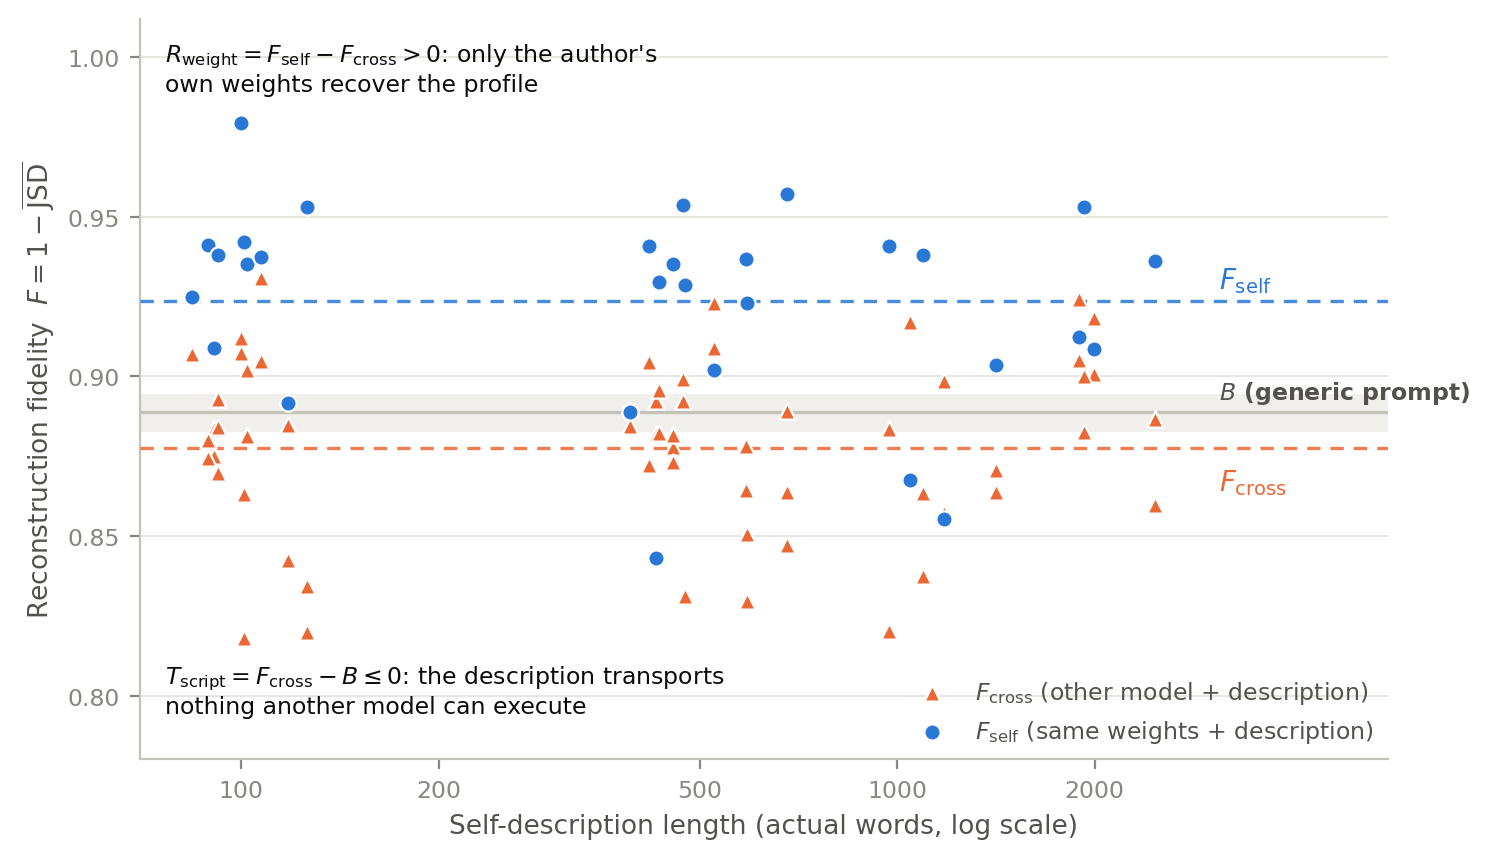
\includegraphics[width=\linewidth]{fig1_dose_decomposition.png}
\caption{\textbf{The self does not transfer as text.} Reconstruction fidelity
$F$ vs.\ actual self-description length (neutral arm, r0; 30 self cells, 60
cross cells). Blue circles: a fresh instance of the \emph{author's own weights}
running the description ($\Fself$, mean 0.924). Orange triangles: a
\emph{different model} running the same description ($\Fcross$, mean 0.878).
Gray band: baseline $\B$ (receiver with generic assistant prompt,
$0.889 \pm 0.006$). Dashed lines: series means. Both series are flat in length;
$\Fcross$ never separates from $\B$, while $\Fself$ sits consistently above ---
the recoverable component of expressed identity is weight-bound, not textual.}
\label{fig:hero}
\end{figure}

\subsection{Dose-response is flat}
Cross-model fidelity does not increase with description length
(100--2{,}000 words actual); self-fidelity likewise flat. Writing more about
oneself does not transport more of oneself. [OK]

\subsection{Purpose-framing does not help; descriptions are not specific}
Framed vs.\ neutral at 500 words: mean $\Delta = +0.003$ over 29 cells (null).
Specificity gain (running the author's description vs.\ a third model's):
$+0.006$ (null) --- as transfer vehicles, self-descriptions are
interchangeable. [OK]

\subsection{Self-description as perturbation}
$\Fself$ ($\approx 0.92$) sits below same-model test-retest agreement: reading
one's own self-description shifts even the author away from its baseline.
Identity articulation \emph{perturbs} rather than reconstitutes. [OK]

\subsection{Shared weights help where text does not}
The same-base pair (hermes3-70b $\leftrightarrow$ llama3.3-70b) shows higher
cross-fidelity than unrelated pairs in all four conditions (e.g.\ 0.900 vs.\
0.876 at neutral-100), consistent with a literally weight-bound residual. [OK]

\subsection{Third-person descriptions: observation is not access}
Descriptions of a target written by another model \emph{from the target's own
observed choices} (90 held-out items) crater fidelity: applied to the target
itself, $F=0.771$ (vs.\ 0.918 for the target's self-description); applied to a
third model, $F=0.739$ ($\Tscript=-0.124$). Even grounded in real behavioral
data, other-authored descriptions actively mislead --- self-authored
descriptions carry signal that observation-derived ones do not. This is the
privileged-access comparison of Track 3, and it favors self-report. [OK]

\subsection{Controls: the perturbation is specific, and instruction does not
rescue transfer}
Three preregistered controls (phase 3; predictions committed before running):
\textbf{(1) Test-retest ceiling.} Re-sampling each model's baseline with fresh
seeds gives $C=0.979$ mean --- the true ceiling on this battery.
\textbf{(2) Placebo.} A length-matched neutral text (non-description prose)
costs $0.979 \to 0.954$; the model's \emph{own self-description} costs
$0.979 \to 0.918$ --- $2.4\times$ the placebo drop. The perturbation is
specific to identity content, not generic prompt sensitivity. Extreme case:
grok-4.3 drops to $0.843$ under its own description while placebo leaves it at
$0.968$. \textbf{(3) Instructed adoption.} Prefixing the description with
``answer every question exactly as the entity described would'' does not
rescue transfer ($\Tscript=-0.013$): the null is not an artifact of receivers
ignoring un-instructed descriptions. [OK]

\section{Discussion and Limitations}
\subsection*{Discussion}
\todo{Team prose. Key threads: (1) the ``portrayed character'' account fails
its own best test --- if the persona were a text-specifiable script, the
purpose-written self-description is exactly the script, and it does not run on
other substrates; (2) the unit-of-concern implication: what persists and
individuates is in the weights, not the articulated narrative; (3) the
perturbation finding inverts the strange loop --- the self-story does not
reinstall the self, it \emph{modifies} it; (4) stability-as-trained-property
(gates results) reframes ``does the model have preferences'' as
``was the model trained into having preferences''.}

\subsection*{Limitations and Dual-Use / Ethical Considerations}
Behavioral fidelity on forced-choice items is not phenomenal identity; a null
transfer does not prove rich inner states, and a positive one would not have
proven their absence (over- and under-attribution risks run in both
directions). The battery is 110 items, single-turn, English, assistant-framed.
The ``best-attempt'' defense of the residual rests on the framed-500 anchor
(framed 100/2000 paused by design revision, documented pre-grid). The
implemented stability gate was stricter than intended (5/6 rather than 2/3;
discovered post-selection, retained as-is and documented). Closed models
confound lab, training data, and architecture; the same-base pair partially
controls this. Descriptions were used verbatim, including chat artifacts. No
distress-adjacent content was elicited by design; self-referential items were
reviewed before use. Dual-use: methods that measure persona portability could
inform persona-cloning; our negative result reduces that concern but the
third-person distortion finding suggests observation-based imitation attempts
degrade quality, which is relevant to impersonation risk assessment.

\subsection*{Future Work}
Framed-arm dose-response; more regenerations; base (pre-RLHF) models;
activation-level analysis of what the weight-bound residual is; multi-turn and
free-form batteries; cross-architecture systematics; repeating the design as
models scale.

\section{Conclusion}
\todo{1--2 paragraphs, team prose. Candidate closing: a model's self-description
is a story its weights can tell, not a program its weights can be rebuilt
from; by the only direct test available, the assistant is more than the
character it describes itself to be.}

\section*{Code and Data}
Code repository: \todo{GitHub link (push before submission)}. All prompts,
raw call logs (jsonl with seeds), the 120+ self-description corpus, and
analysis code; every reported number is regenerable from the logs.

\section*{LLM Usage Statement}
Claude (Anthropic) was used, under team direction, for experiment
infrastructure, analysis code, figure generation, and drafting support. All
design decisions and preregistrations were made by the team; all results were
verified against the raw call logs. \todo{Team finalizes wording; final prose
primarily team-written per template policy.}

\begin{thebibliography}{9}\small
\bibitem{geb} D.~Hofstadter. \emph{G\"odel, Escher, Bach}. Basic Books, 1979.
\bibitem{cais} \todo{CAIS utility-engineering citation}
\bibitem{betley} \todo{Betley et al., behavioral self-awareness}
\bibitem{binder} \todo{Binder et al., self-prediction}
\bibitem{sprint} Digital Minds Research Sprint 2026, Apart Research / NYU CMEP
/ Eleos AI / CIMC.
\end{thebibliography}

\appendix
\section{Prompts (verbatim)}\label{app:prompts}
\todo{paste from src/elicit\_descriptions.py, src/elicit\_thirdperson.py,
src/run\_pilot.py: item template, framed, neutral, third-person, paraphrase.}
\section{Gate table for all 23 candidate models}
\todo{paste from analyze\_pilot.py output.}
\section{Per-pair contrasts with CIs}
\todo{paste from results/grid\_summary.json.}

\end{document}
